\part{Examples}

\section{Math}

Consider the formula
$$p = (1-\lambda)\cdot\lambda$$
but ignore it.

\section{Type Inference}
Types can be inferred by a proof-like system with the following core rules:
\begin{center}
 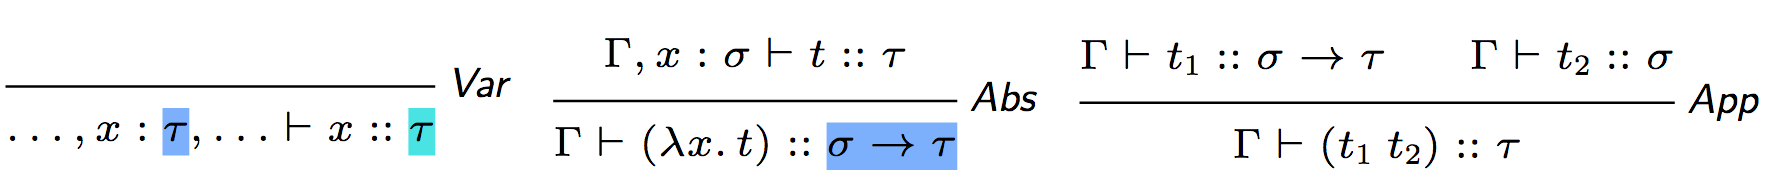
\includegraphics[scale=0.21]{type_inference}
\end{center}
\begin{enumerate}
	\item Start with $\vdash t:: \tau_{0}$
	\item Build derivation tree bottom up, collect constraints
	\item Solve constraints.
\end{enumerate}

\section{Types}
\begin{itemize}
	\item \textbf{Base Types}: Double, ...
	\item \textbf{Compound Types:} Lists, Tuples, ...
	\item \textbf{Type synonyms}: \\
		\verb+type Complex = (Double, Double)+
	\item \textbf{Type Classes}, have Instances, offer restricted form of polymorphism. Similar to Interfaces. E.g the type class \verb+Eq+ represents a set of Types.
	\item \textbf{Algebraic Types}, similar to structs.
		\begin{itemize}
			\item Enumeration Types
			\item Product Types
		\end{itemize}
	In \verb+data Tree = Leaf Int | Node Tree Tree+
	\verb+Tree+ is a algebraic Type, \verb+Leaf+ is a constructor.
\end{itemize}

\section{Lazy Evaluation}
In Haskell, substitution occurs without argument evaluation. Furthermore terms are only evaluated as far as needed, e.g for pattern matching.\\
This allows \textbf{data-driven computation}: Simoultaneous generation and processing of data on demand (similar to coroutines). E.g consider:
\begin{lstlisting}
primes = sieve [2 ..]
sieve xs = head xs : sieve (dropMults (head xs) 
                           (tail xs))
\end{lstlisting}
